
{\cmerge} is a {\CPP} class that performs merging of 2D clusters, and is an application of {\cmalgo} algorithm classes that are inherit from {\cbalgo}, the algorithm base class. In a few sentences, {\cmerge} perform merging by looping over all possible 2D cluster pairs among the given set of clusters. For each pair, {\ttfamily Bool()} function of both merging and prohibit {\cmalgo} are called to inspect possible 2D cluster merging. It uses {\cbkeeper} to keep track of which pair of clusters are merged. For details of {\cbalgo} and {\cbkeeper}, see Sec.\ref{sec:fmwk:base:cbalgo} and Sec.\ref{sec:fmwk:base:cbk} respectively. The overall process stream diagram is shown in Fig.\ref{sec:fmwk:base:cmerge_stream} which we keep referring in this section.

\subsection{Why {\cmerge}?}
Why using {\cmerge}? Why not just writing a program that does everything from scratch?
Be my guest and write your code! That might inspire a better design or strategy toward merging. 
That being said, there are a few reasons to use {\cmerge}.

\paragraph{Task Outside Merging Decision:}
{\cmerge} The core part of merging is to compare 2 clusters and make a decision to merge or not. Outside this process, however, there is a non-negligible overburden of running such algorithm such as (1) keeping track of which cluster pairs are merged and (2) optimizing the loop process of cluster pair comparison. {\cmerge} does those tedious jobs while out-sourcing the decision making to an independent {\CPP} algorithm class that inherit from {\cbalgo}. 

\paragraph{Easy Development via Modulated Design:}
Because {\cmerge} outsource an independent algorithm class to perform merging of a cluster pair, it supports modulated code design. Accordingly each {\cmalgo} class becomes a pure algorithm class. This makes a code development very easy because a new algorithm can be written without re-writing the I/O or book-keeping part. Also it makes life easy to compare different algorithms: you can simple change which algorithm to be attached to {\cmerge} at run-time, and this avoids re-compilation or re-writing of code.

\paragraph{X-Framework Implementation}
{\cmerge} does not use data product type specific to an analysis framework (for instance {\larlight} or {\larsoft}), so it can be ported easily among different frameworks. That means {\cmalgo} developed by one person in one analysis framework can be shared among other frameworks (assuming an algorithm developer follows x-framework design pattern).\\

\subsection{How Does It Work?}
\label{sec:fmwk:cmerge:how}
The core part of decision making is simple: provided 2 clusters, decide whether they should be merged or not.
This is done through {\cmalgo::Bool()} function call:
\begin{lstlisting}
  virtual bool Bool( const cluster::ClusterParamsAlg &, 
                       const cluster::ClusterParamsAlg &)
\end{lstlisting}
If the return is {\ttfamily true}, two clusters are merged. Else not.
This is ilustrated in Fig.\ref{sec:fmwk:cmerge:merge_example}.

\begin{figure}[ht]\begin{center}
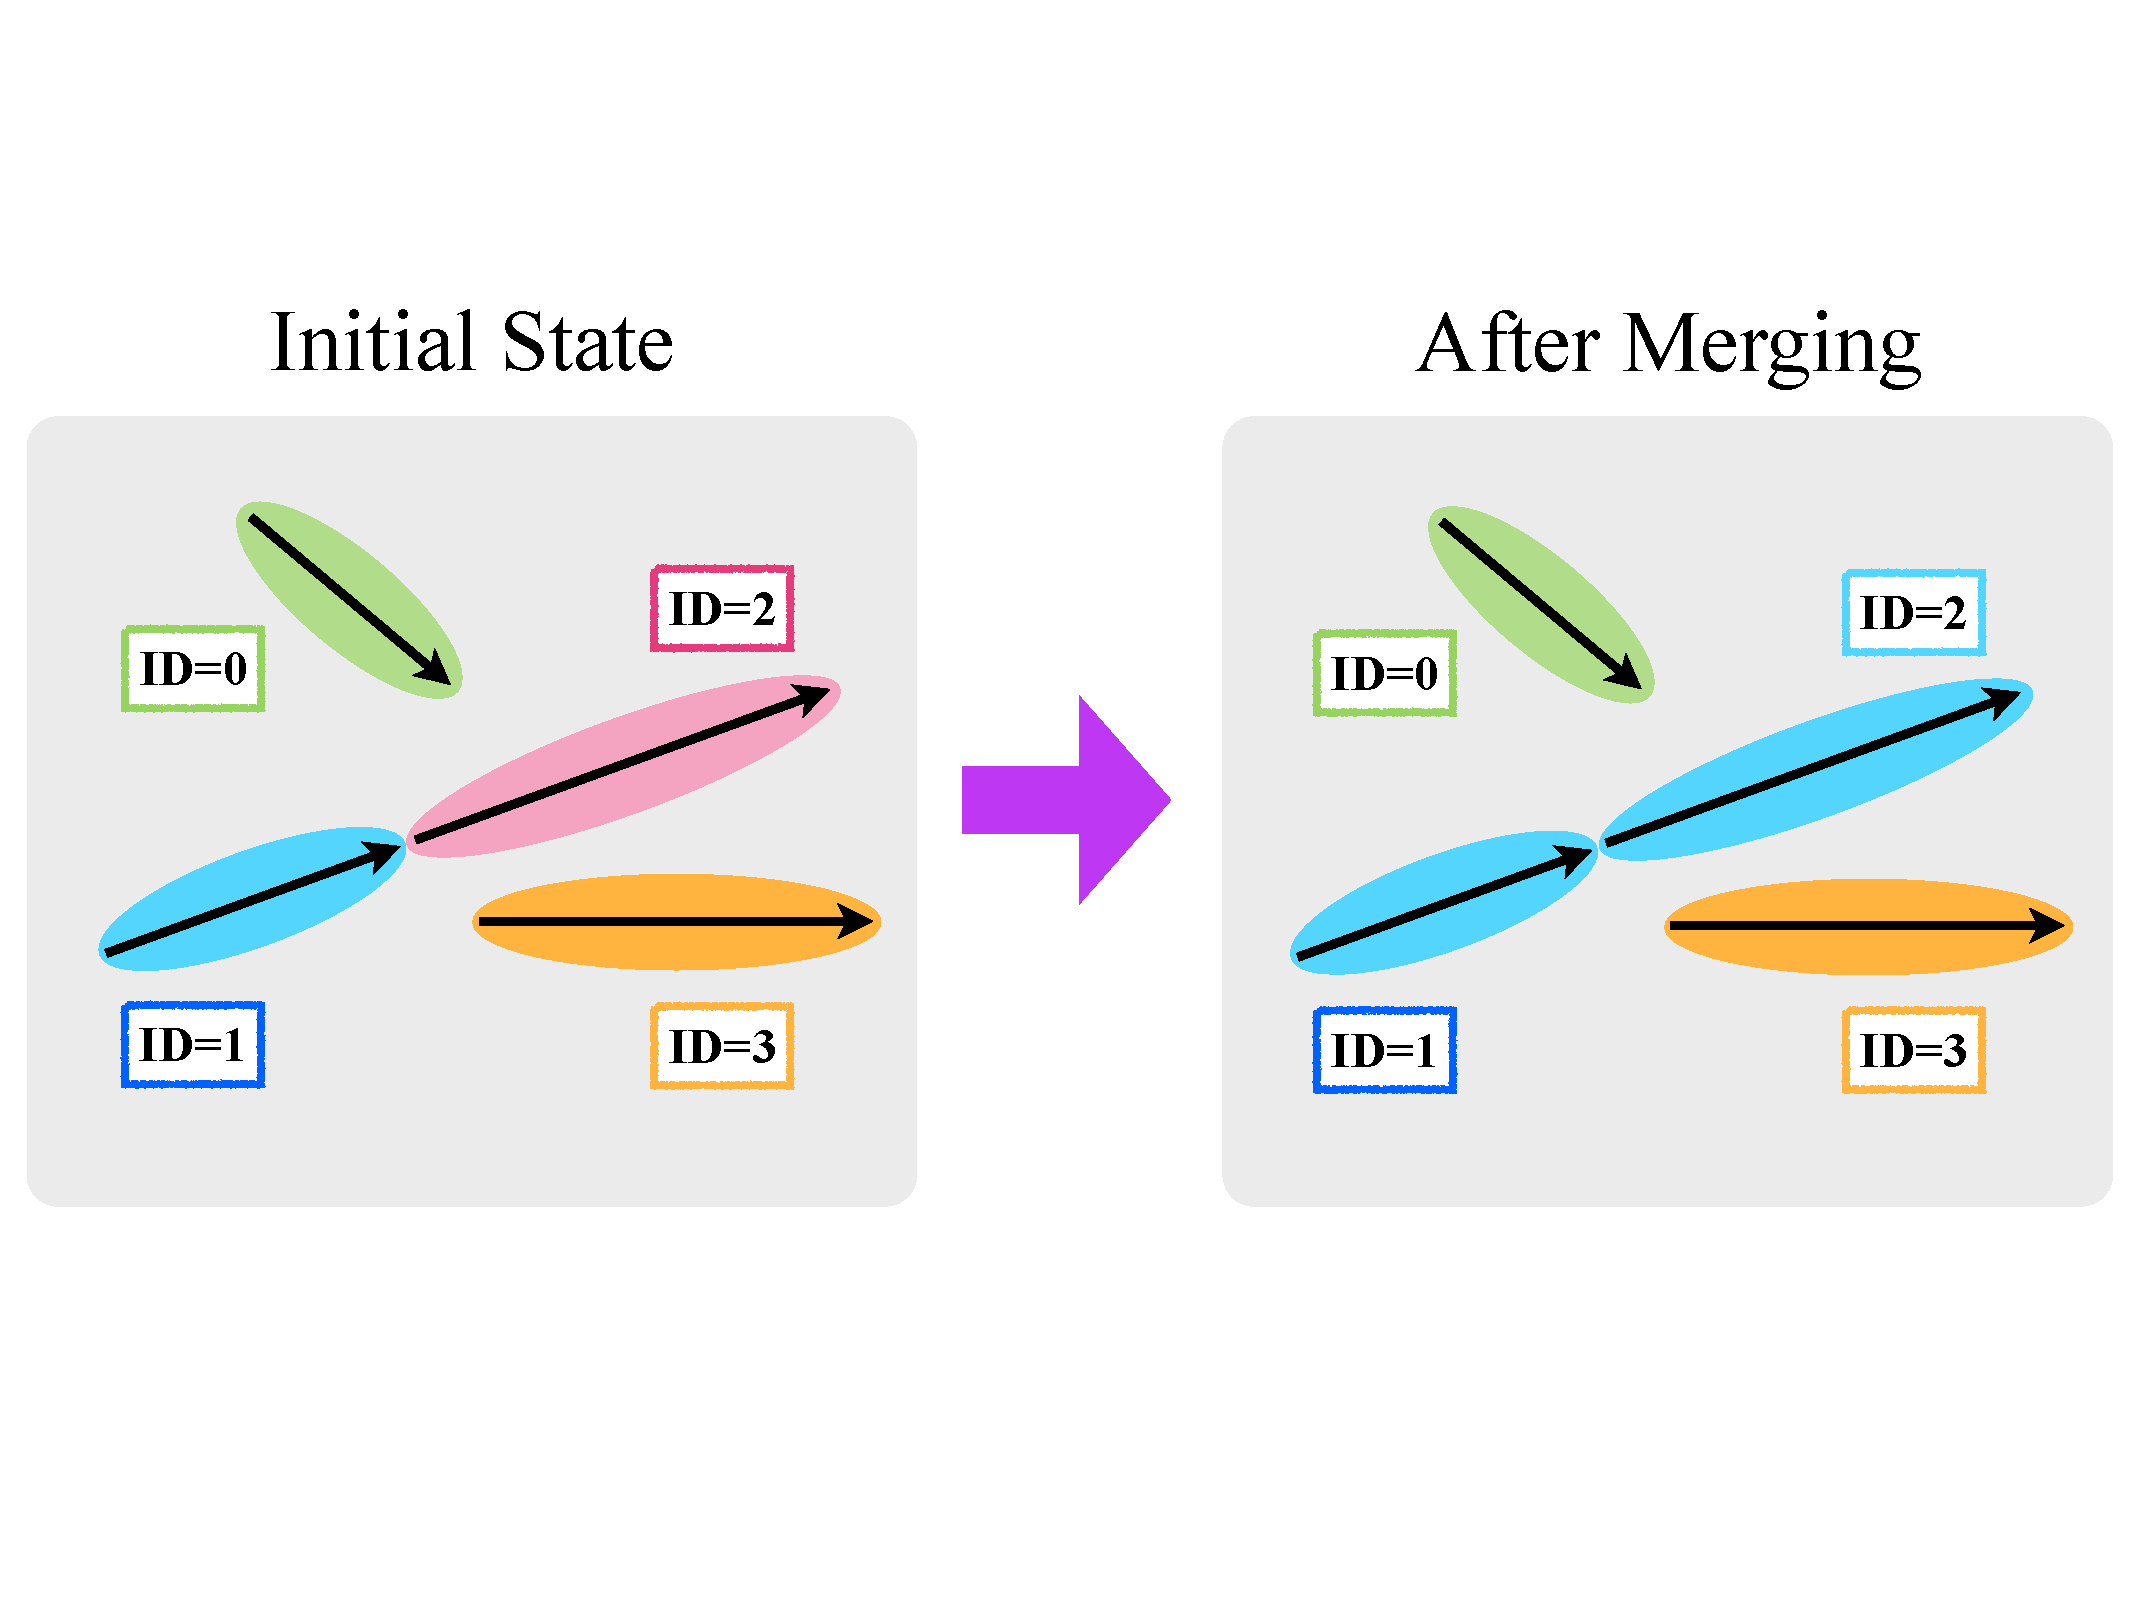
\includegraphics[width=13cm]{./src/Pictures/MergeExample.pdf}
\caption{Example of 2D clusters in a plane before and after merging attempt. Each oval represents a cluster with cluster 2D axis shown in a black solid arrow. The direction of an arrow represents the direction of a cluster development. Each cluster is labeled with an input cluster ID number while the oval color represents distinct output cluster group. Left: initial state with 4 input clusters. Right: example output after running a merge loop over cluster pairs. }
\label{sec:fmwk:cmerge:merge_example}
\end{center}\end{figure}
{\cmerge} takes care of creating a loop over all possible pairs of 2D clusters and calling the above function of {\cmalgo} for merging.
In the process, book-keeping of which pairs to be merged is recorded using {\cbkeeper}.

\begin{figure}[ht]\begin{center}
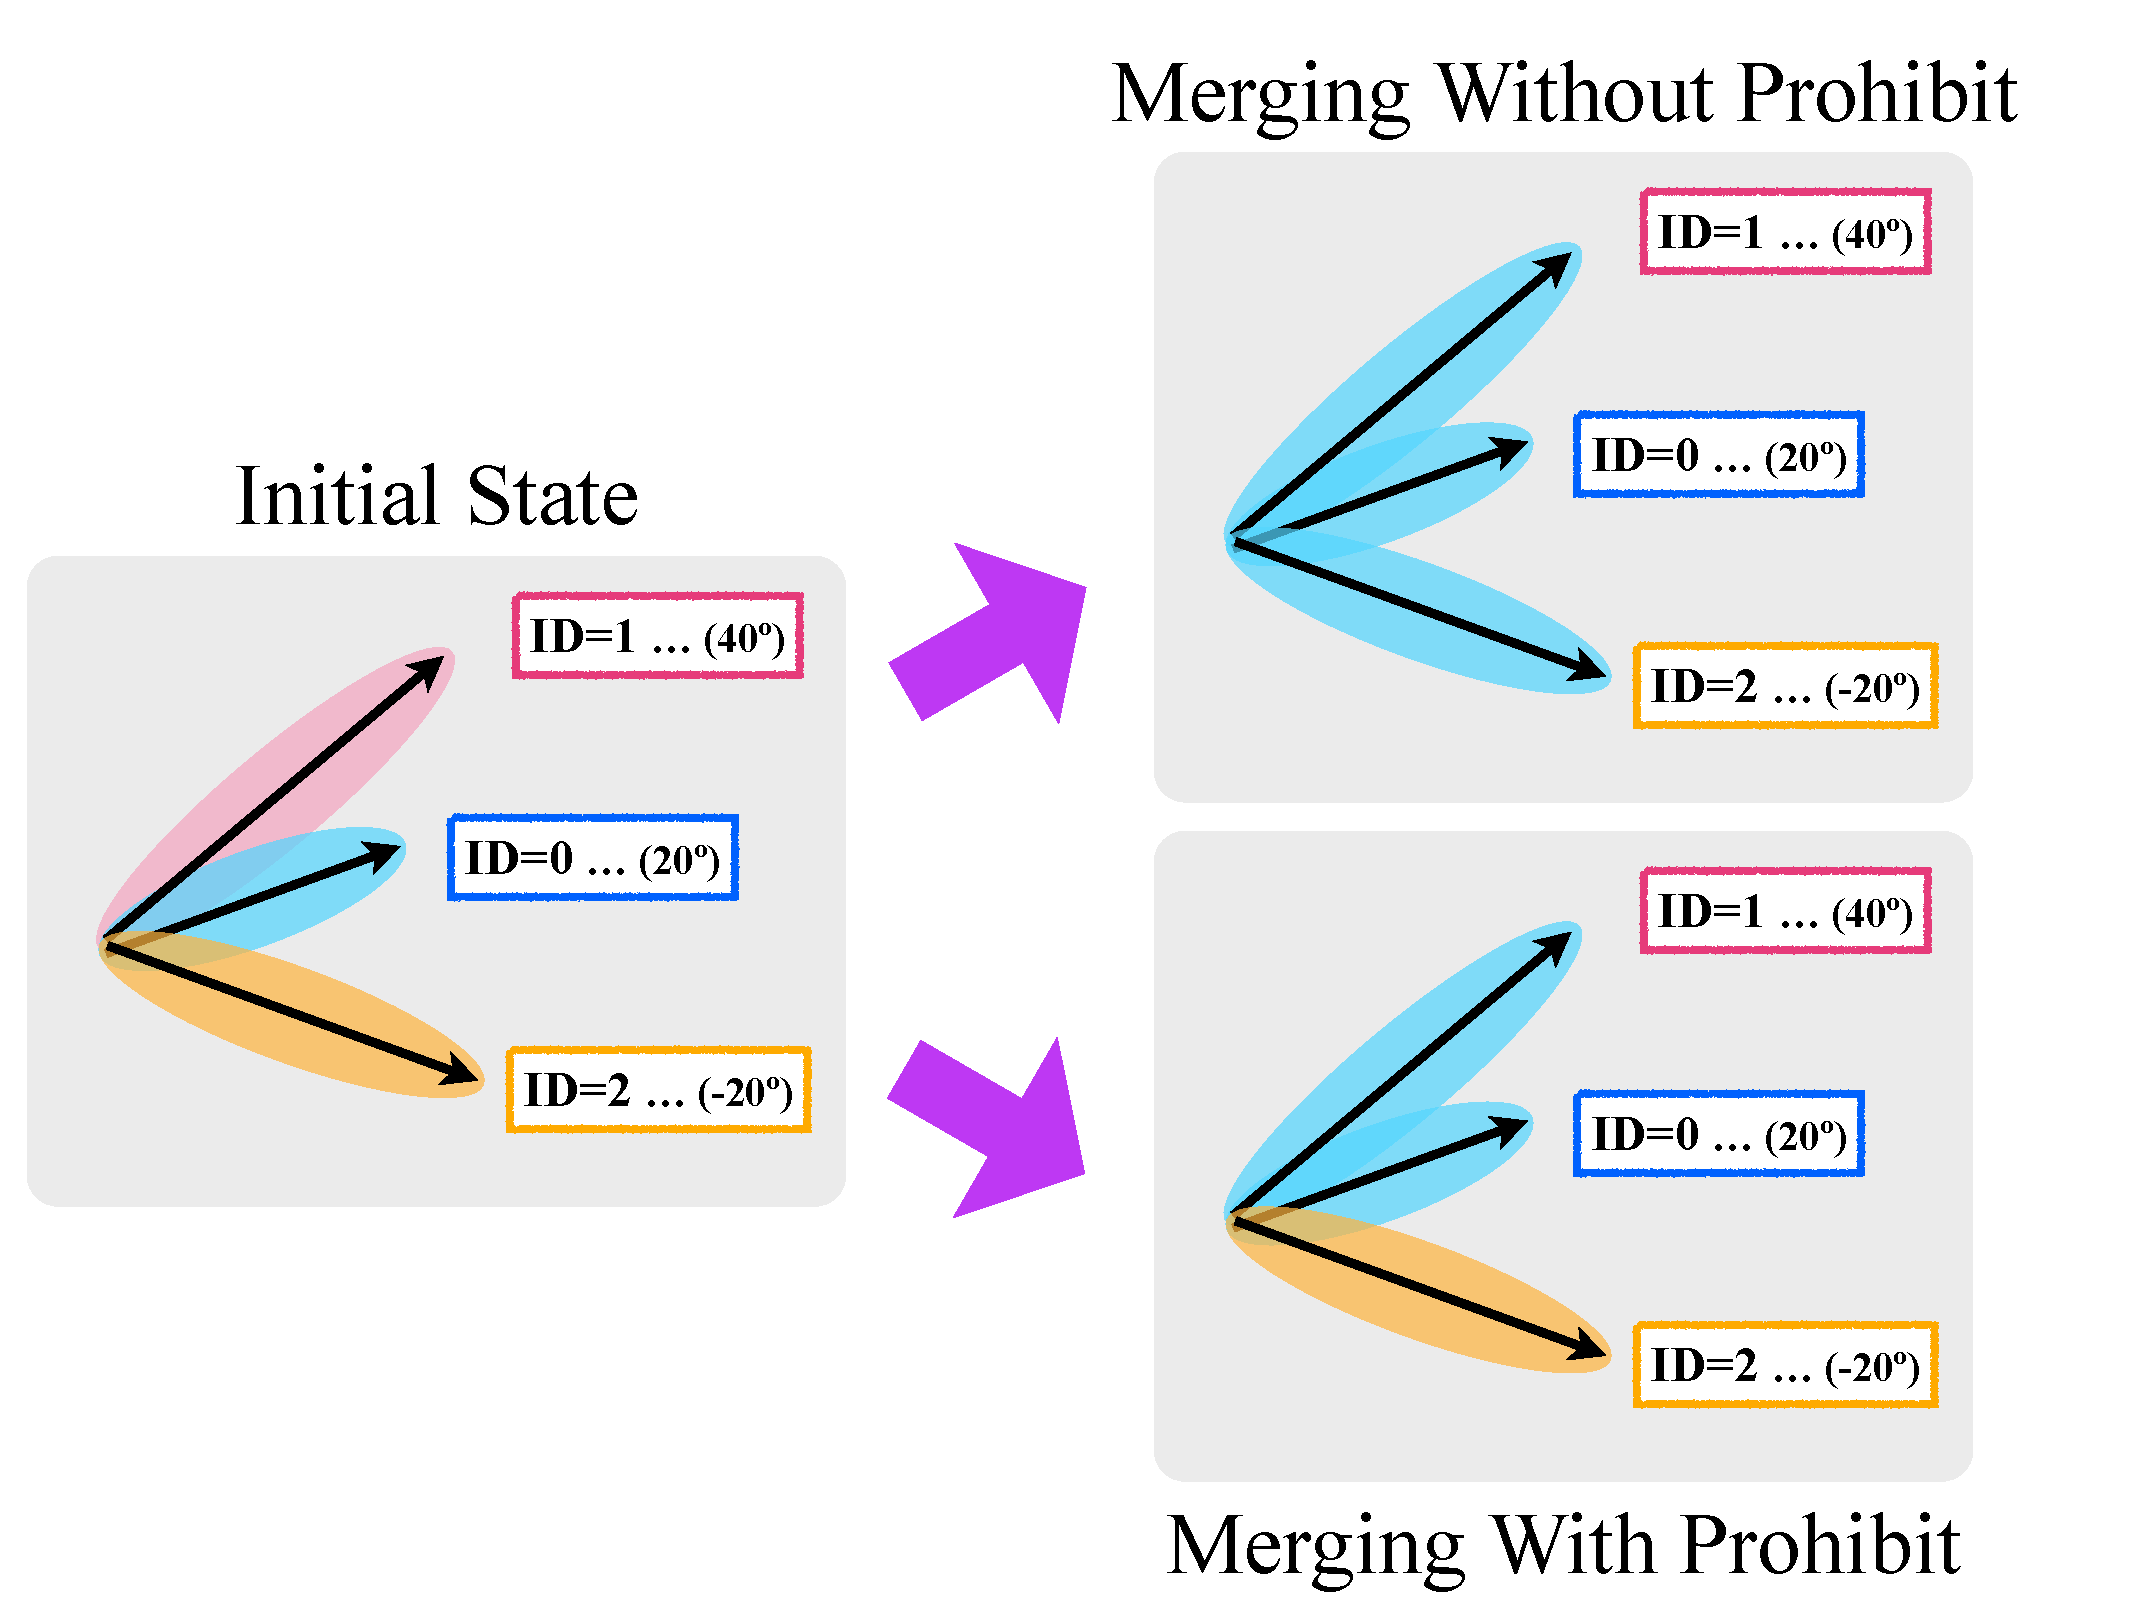
\includegraphics[width=13cm]{./src/Pictures/MergeProhibitExample.pdf}
\caption{Example of how prohibit algorithm works. Each oval and solid arrow represents a 2D cluster with its direction while the color represents distinct output (merged) cluster. Input cluster index (ID) is shown in the label with the cluster 2D angle. Right-top shows an output of running {\cmalgo} that merge clusters with angle difference within 40 degrees. Right-bottom shows an output of the same {\cmalgo} for merging but with another {\cmalgo} that prohibits merging of clusters with angle difference larger than 40 degrees.}
\label{sec:fmwk:cmerge:merge_prohibit_example}
\end{center}\end{figure}
Let us consider a case of two merged pairs that shares the same input cluster ID. As described in Sec.\ref{sec:fmwk:base:cbk}, {\cbkeeper} combines two pairs of 2D clusters in such case (see Fig.\ref{sec:fmwk:base:cbk}). This could be problematic sometimes. For instance, consider an example {\cmalgo} that combines two clusters if their start points are very close and the angle between two clusters are within 40 degrees. Further assume we have 3 input clusters that share the start point but have different angles at 20, 40, and -20 degrees. For convention these have input cluster ID 0, 1, and 2 respectively. This example algorithm would conclude pairs (0,1) and (0,2) but not for (1,2). But because merged pairs share cluster ID 0, it ends up all 3 clusters being merged. This is shown in the right-top ilustration of Fig.\ref{sec:fmwk:cmerge:merge_prohibit_example}.

This could be a problem, or may not be: this can be only answered by the algorithm author.
The way to avoid this in {\cmerge} is to implement another {\cmalgo} as {\it merge-prohibit}, or simple {\it prohibit} algorithm.
When prohibit algorithm is provided, {\cmerge} first run over all cluster pairs and execute {\ttfamily Bool()} function to find all cluster pairs that are prohibited to merge.
Then {\cmerge} run over the same set of cluster pairs except for those are prohibited to be merged.
The right-bottom ilustration of Fig.\ref{sec:fmwk:cmerge:merge_prohibit_example} shows how prohibit algorithm affects the result.

The prohibit rule is also inherited to merged cluster pairs. For instance, consider input clusters 0, 1 and 2. The pair (1,2) is prohibited to merge, and (0,1) is found to be merged. Then the merged cluster, (0,1) cannot be merged with 2. That means even if a merge algorithm finds (0,2) to be merged, it cannot be because the prohibit rule is inherited from cluster 1 when 0 and 1 aremerged. This feature brings up a question: what determines 0 to be merged with 1 rather than 2? If the merge algorithm is executed on the pair (0,2) first, then the result would have been different. So what determines a different outcome is an order of cluster pairs in the loop of merging inspection. There are different ordering options available in {\cmerge}. Currently available options are defined as {\enum} type in {\cmerge} class, {\ttfamily CMergePriority\_t} which include following values.
\begin{itemize}
\item[] {\ttfamily kIndex}
  \begin{itemize}
    \item From the smaller to larger input cluster ID, basically following input cluster set ordering
  \end{itemize}

\item[] {\ttfamily kPolyArea}
  \begin{itemize}
    \item From the clusters with smaller polygon area to the larger
  \end{itemize}

\item[] {\ttfamily kChargeSum}
  \begin{itemize}
    \item From the clusters with smaller charge sum to the larrger
  \end{itemize}

\item[] {\ttfamily kNHits}
  \begin{itemize}
    \item From the clusters with smaller number of hits to the larger
  \end{itemize}

\end{itemize}
The ordering parameters including all listed above are taken from {\ttfamily cluster\_params} member attributes.
If more useful parameter is found, one should make a request to make it available. 
It is very simple to implement in {\cmerge}.

In summary, {\cmerge} uses one {\cmalgo} instance for merging and another for merge-prohibit. A possible ambiguity of which cluster pairs to be merged in the presence of prohibited pairs is resolved by defining a priority for cluster pairs in the merging attempt. 

\subsection{Process Flow for Cluster Merging}
\label{sec:fmwk:cmerge:process_flow}
An overall process flow diagram is already shown in Fig.\ref{sec:fmwk:base:cmerge_stream}, so here we describe slightly more details in texts by breaking down into 5 blocks.
\begin{enumerate}
\item Event Preparation
  \begin{itemize}
    \item[] {\cmerge} receives an input cluster in terms of a set of {\pxhit} (see Sec.\ref{sec:fmwk:cmerge:input}). Then it creates {\cpan} instance for each cluster, and calls {\cmalgo::EventBegin()} for merging and prohibit algorithms.
  \end{itemize}

\item Iterative Merge Operation
  \begin{itemize}
    \item[] A loop over cluster pairs for prohibit (if provided) and merge {\cmalgo} can be configured to repeat until no newly merged cluster is found. This is shown in Fig.\ref{sec:fmwk:cmerge:iterative_stream}. If a user does not configure to choose iterative approach, iteration will not happen even if there is a newly merged cluster in the output.
  \end{itemize}

\item Prohibit {\cmalgo} Loop Over Cluster Pairs
  \begin{itemize}
    \item[] See Fig.\ref{sec:fmwk:cmerge:iterative_stream}. Only occurs if prohibit algorithm is provided by a user (optional). Records which cluster pair to be prohibited for merging using {\cbkeeper}.
  \end{itemize}

\item Merge {\cmalgo} Loop Over Cluster Pairs
  \begin{itemize}
    \item[] See Fig.\ref{sec:fmwk:cmerge:iterative_stream}. The algorithm's {\ttfamily Bool()} is not executed for a subject pair of clusters if (a) they are prohibited for merging or (b) already inspected in the previous process and not merged (i.e. result should not change). This is to save computation time.
  \end{itemize}

\item Merge Clusters
  \begin{itemize}
    \item[] Based on the outcome of merge/prohibit {\cmalgo} algorithms, actual merging is performed at this step. It creates a new set of {\cpan} for merged clusters. For clusters that are not merged, {\cpan} instance is copied from input to save {\cpan} computation time.
  \end{itemize}

\end{enumerate}

\begin{figure}[ht]\begin{center}
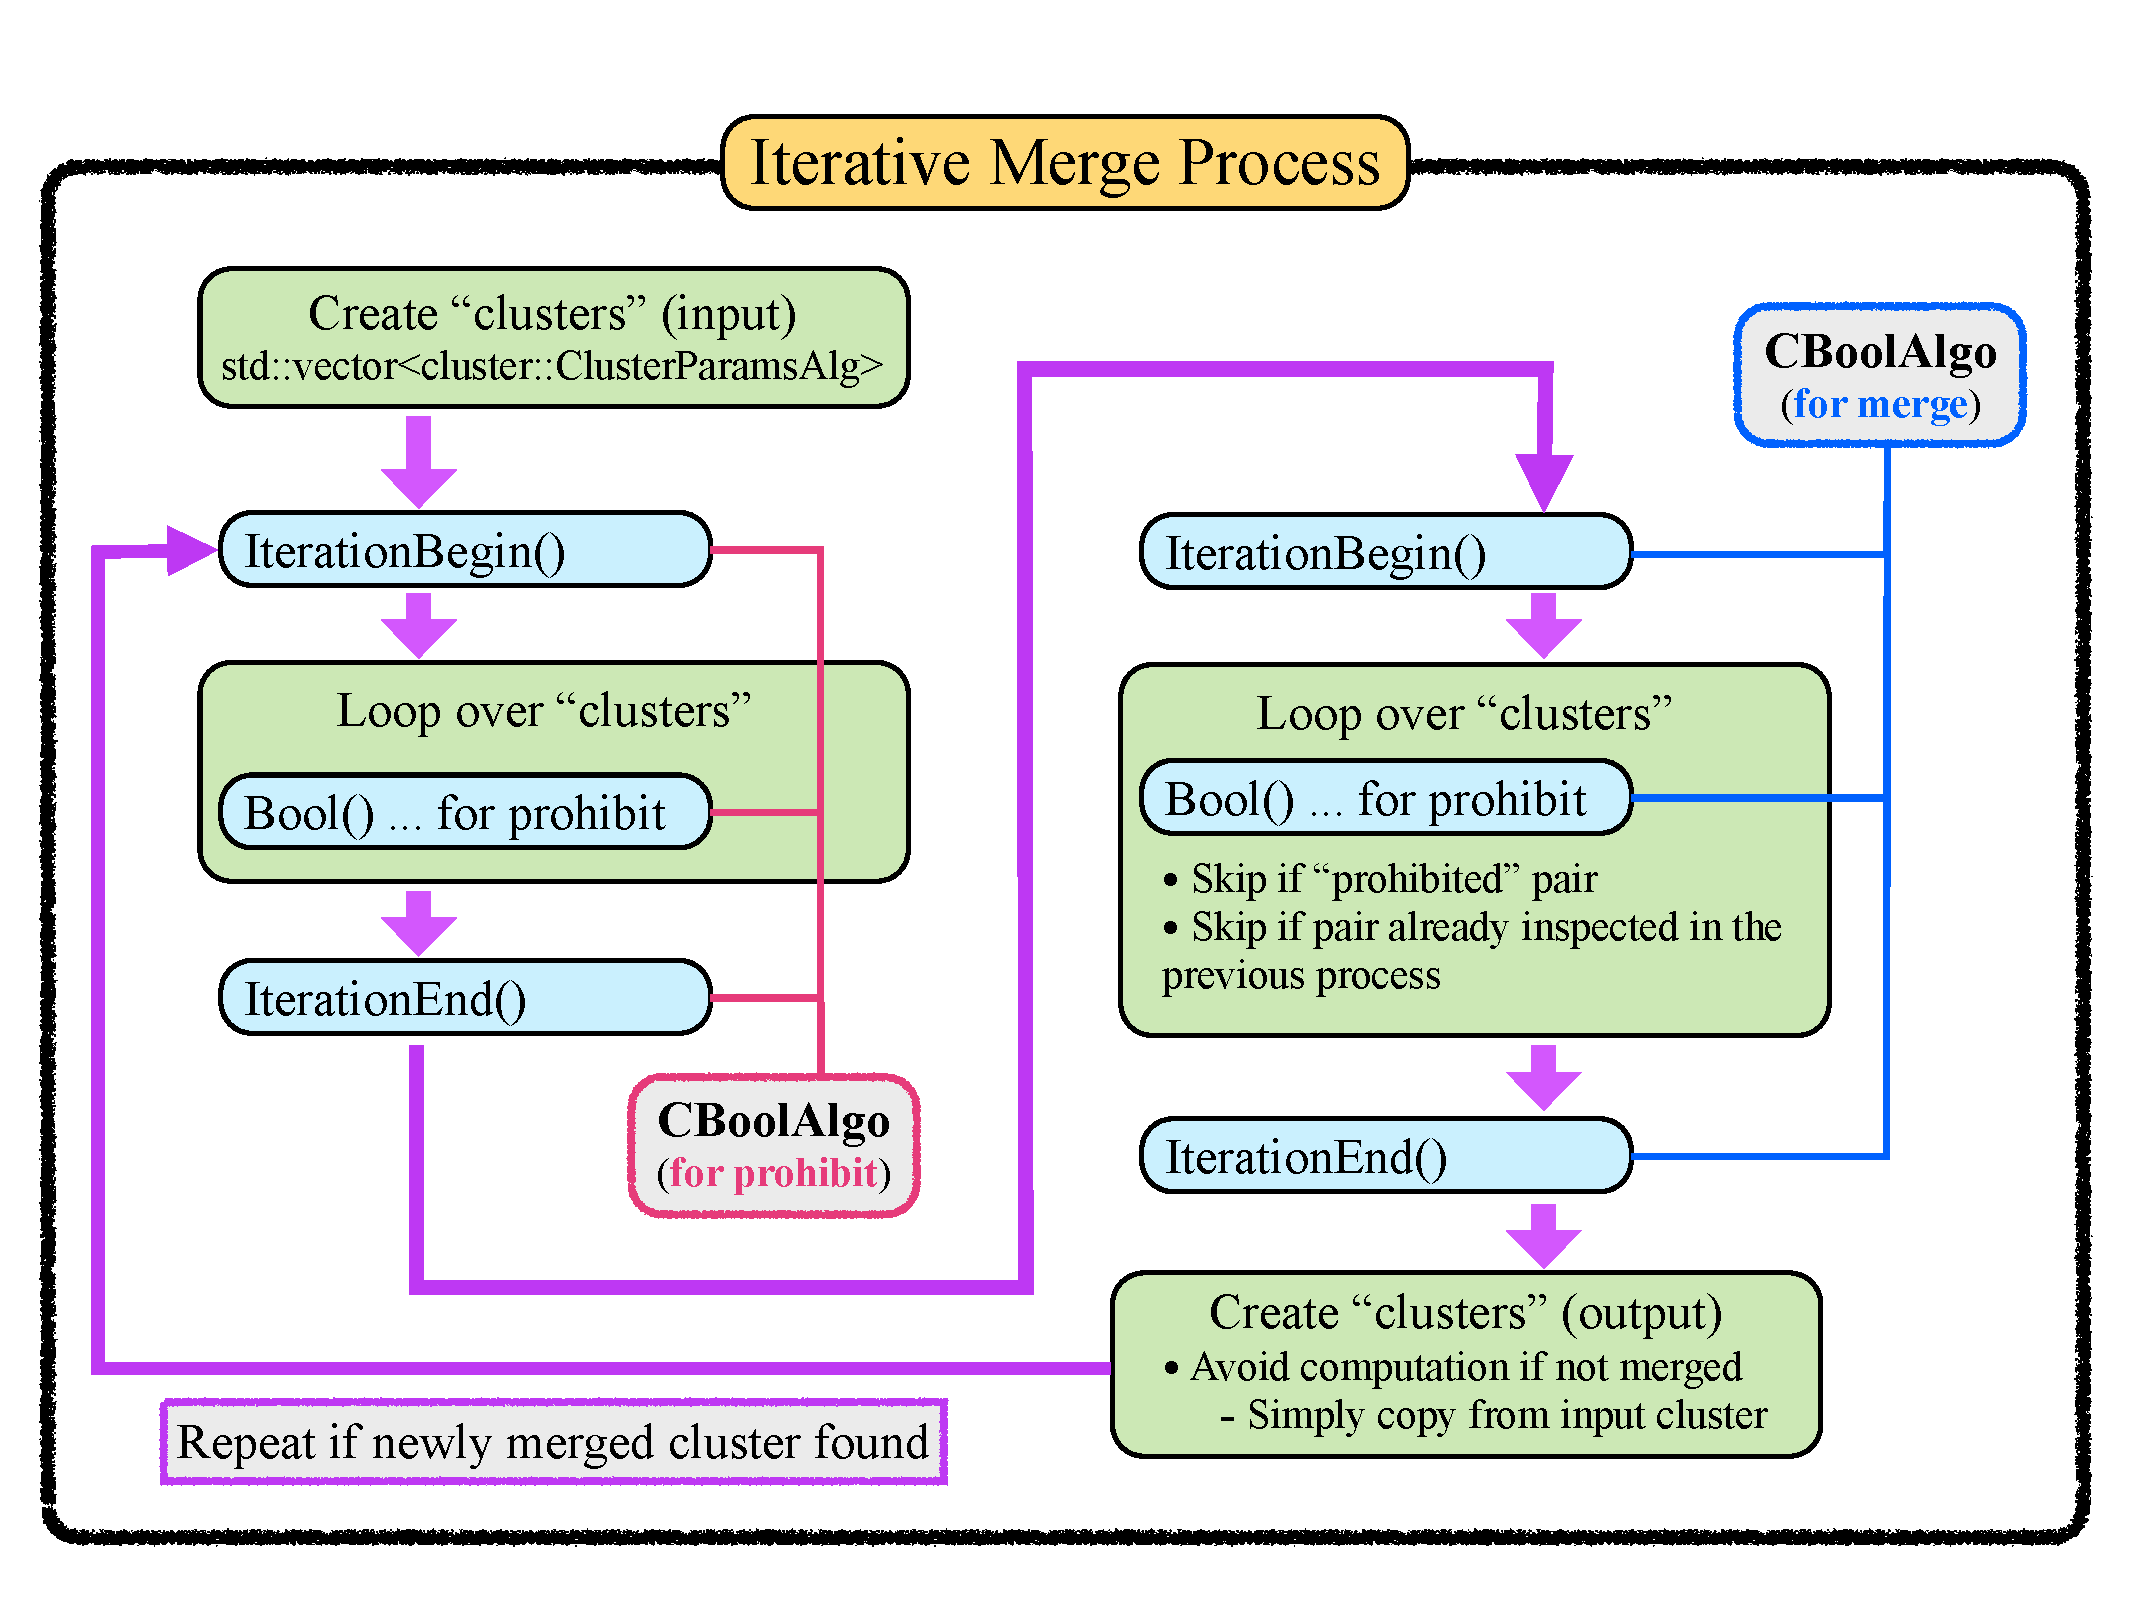
\includegraphics[width=13cm]{./src/Pictures/IterativeMergeApproach.pdf}
\caption{Illustration of how iterative merge approach is processed. Internally a loop over cluster pairs for prohibit and merge algorithm are repeated if (a) user configured to use an iterative approach and (b) newly merged cluster is found.}
\label{sec:fmwk:cmerge:iterative_stream}
\end{center}\end{figure}


\subsection{Setting an Input 2D Clusters}
\label{sec:fmwk:cmerge:input}
Input to {\cmerge} is a set of clusters where each cluster is represented as a vector of hits, or more precisely {\ttfamily std::vector<util::PxHit>}. This input can be set by the following function:
\begin{lstlisting}
  void SetClusters(const std::vector<std::vector<util::PxHit> > &)
\end{lstlisting}
where the argument is a vector of 2D clusters. When this function is called, {\cmerge} internally calls
\begin{lstlisting}
  void Reset()
\end{lstlisting}
which initialize previously stored input clusters, output clusters and {\cbkeeper} instance.
Then it creates {\cpan} instance per input 2D cluster using a set of {\pxhit}.
This completes setting (or initiating) the input 2D cluster sets to be used for internal processing.

\subsection{Setting Merge/Prohibit {\cmalgo} Instances}
{\cmalgo} instance is necessary for merging and optional for prohibit. Call the function,
\begin{lstlisting}
  void AddMergeAlg(CBoolAlgoBase* algo)
\end{lstlisting}
to set {\cmalgo} for merging, and 
\begin{lstlisting}
  void AddSeparateAlgo(CBoolAlgoBase* algo)
\end{lstlisting}
to set {\cmalgo} for merge-prohibit.

\subsection{Setting Run Configuration}
There are only 3 run options to configure for {\cmerge}.

\paragraph{Verbosity:} 
There are 5 verbosity levels a user can configure as listed below:
\begin{itemize}
\item[] {\ttfamily kNone}
  \begin{itemize}
    \item No report from {\cmerge}
  \end{itemize}

\item[] {\ttfamily kPerEvent}
  \begin{itemize}
    \item Report made at the end of even processing
  \end{itemize}

\item[] {\ttfamily kPerIteration}
  \begin{itemize}
    \item Report made per merge iteration (see Sec.\ref{sec:fmwk:cmerge:process_flow}). This could be quite verbose.      
  \end{itemize}

\item[] {\ttfamily kPerMerging}
  \begin{itemize}
    \item Report made per {\cmalgo::Bool()} execution (see Sec.\ref{sec:fmwk:cmerge:process_flow}). This is even more verbose than {\ttfamily kPerIteration}.
  \end{itemize}

\end{itemize}
These are {\enum} type, {\ttfamily CMergeMSGLevel\_t}, defined under {\cmerge} class. 
The verbosity level can be set by the function:
\begin{lstlisting}
  void DebugMode(CMergeMSGLevel_t level)
\end{lstlisting}

\paragraph{Iterative Approach:}
As described in Sec.\ref{sec:fmwk:cmerge:process_flow}, {\cmerge} can be configured to attempt iterative approach for merging. This can be enabled by the following function call.
\begin{lstlisting}
  void MergeTillConverge(bool)
\end{lstlisting}
Providing {\ttfamily true} as an argument will enable this option. Disabled if {\ttfamily false} is provided.

\paragraph{Merge Priority:}
As described in Sec.\ref{sec:fmwk:cmerge:how}, ordering of cluster pairs for merging inspection matters to the result.
Options are also described in the same section. This can be set by the following function.
\begin{lstlisting}
  void SetMergePriority(CMergePriority_t level)
\end{lstlisting}

\subsection{Execute Merging}
To execute merging, simply call
\begin{lstlisting}
  void Process()
\end{lstlisting}

\subsection{Obtaining Result}
There are two kinds of results that may be useful for a user. First is a resulting (i.e. merged) set of clusters in terms of {\cpan}. This is useful for further processing as various cluster parameters are already computed as a part of {\cpan}. You can execute
\begin{lstlisting}
  const std::vector<cluster::ClusterParamsAlg>& GetClusters() const
\end{lstlisting}
to obtain such result set.

Second is a mapping of input cluster IDs (i.e. index) to the output (merged clusters). 
As described in Sec.\ref{sec:fmwk:base:cbk}, this can be easily obtained through {\cbkeeper} instance.
You can obtain the {\cbkeeper} instance held by {\cmerge} through the following function.
\begin{lstlisting}
  const CBookKeeper& GetBookKeeper() const
\end{lstlisting}
